\chapter{Resultados Obtidos}
\label{cap:ResultadosObtidos}

Conforme visto no capítulo 5 através da tabela \ref{tab:questaoNegocio}, foram elencadas 5 questões que os especialistas de domínio entenderam ser necessárias. A partir do desenvolvimento do modelo OLAP, detalhado na primeira seção do capítulo 5, e dos processos de carga através dos \emph{scripts} de ETL elaborados dentro do trabalho, foi possível a criação do cubo e suas respectivas dimensões dentro do \emph{Microsoft Analysis Services}. Durante o período de criação das dimensões e do próprio cubo, foram realizadas reuniões com os especialistas para adequar o modelo OLAP de maneira que fosse possível endereçar todos os pontos levantados. 

Após a primeira execução e exibição dos resultados no cubo, os especialistas observaram que a FEB média para o ligante Triclosano estava positiva. Inicialmente acreditou-se que era um problema da carga mas, depois de avaliar os resultados da docagem diretamente na base de dados das conformações, viu-se que boa parte dos resultados da melhor FEB para o ligante Triclosano era realmente positivo. Os especialistas então pediram que todo e qualquer FEB positivo fosse substituído pelo valor 0, conforme descrito na seção \ref{sec:IdentificacaoDeMetricas}. Com esta alteração foi necessário realizar uma nova carga dos dados.

Para exibir os resultados e para realizar a composição dos valores e dimensões afim de responder às questões de negócio, foi utilizado o \emph{plug-in} do \emph{Microsoft Excel} para o \emph{Analysis Services}. A figura \ref{fig:questao1} mostra a associação dos agrupamentos para cada uma das conformações, respondendo assim a primeira questão. 

\begin{figure}[h]
        \center
        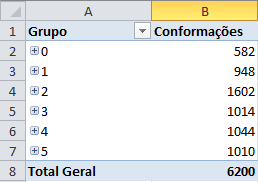
\includegraphics[scale=0.8]{images/Questao1.PNG}
        \caption{Resultado para a primeira questão}
        \label{fig:questao1}
\end{figure}

\newpage

A figura \ref{fig:questao2} exibe o comportamento de cada agrupamento das conformações, levando em consideração a FEB e RMSD médios, respondendo assim a segunda questão levantada pelos especialistas de domínio.

\begin{figure}[h]
        \center
        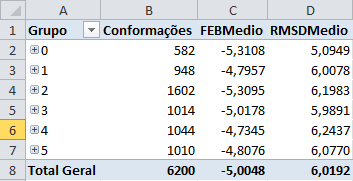
\includegraphics[scale=0.8]{images/Questao2.PNG}
        \caption{Resultado para a segunda questão}
        \label{fig:questao2}
\end{figure}

A figura \ref{fig:questao3} mostra os agrupamentos das conformações por cada número de contato dos resíduos com o ligante, possibilitando levantar qual ou quais possuem maior número de contatos estabelecidos e desta forma respondendo a terceira questão de negócio. 

\begin{figure}[h]
        \center
        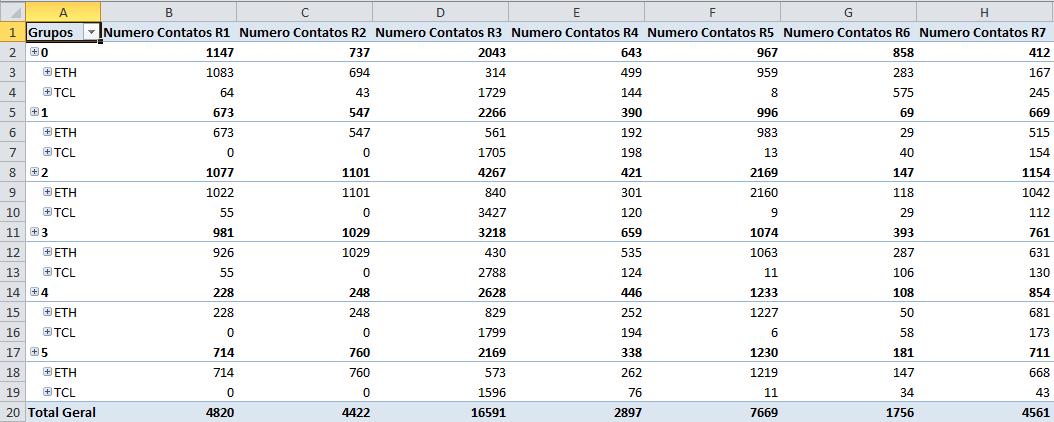
\includegraphics[scale=0.62]{images/Questao3.PNG}
        \caption{Resultado para a terceira questão}
        \label{fig:questao3}
\end{figure}

\newpage

A figura \ref{fig:questao4} mostra qual foi o número de contatos de cada um dos principais resíduos em relação aos agrupamentos das conformações. Esta composição permite identificar quais são os resíduos mais importantes por agrupamento, respondendo assim a quarta questão da tabela \ref{tab:questaoNegocio}.

\begin{figure}[h]
        \center
        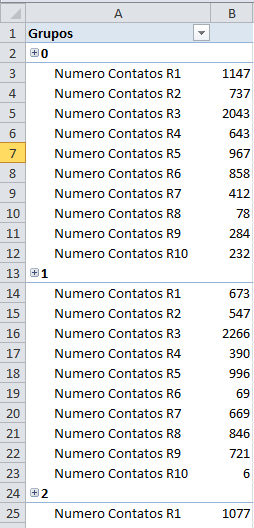
\includegraphics[scale=0.7]{images/Questao4.PNG}
        \caption{Resultado para a quarta questão}
        \label{fig:questao4}
\end{figure}

Para a quinta e última questão, a figura \ref{fig:questao5} exibe qual foi o FEB e RMSD médios para cada um dos agrupamentos, permitindo avaliar quais grupos possuem os melhores resultados para estas métricas.

\begin{figure}[h]
        \center
        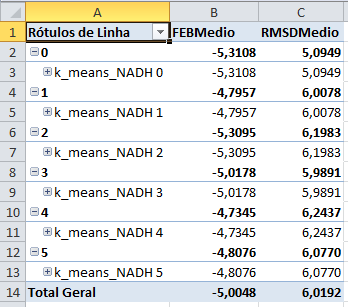
\includegraphics[scale=0.8]{images/Questao5.PNG}
        \caption{Resultado para a quinta questão}
        \label{fig:questao5}
\end{figure}
